Dieser Abschnitt erklärt die Arbeitsweise der implementierten Authentifizierung.

\section{HTTP-Authentifizierung}
Die Authentifizierung für HTTP soll sicherstellen, das die Anfragen eines Benutzers nur bearbeitet werden, wenn dieser dazu berechtigt ist. 
Durch die Feststellung der Identität wird die Sicherheit des Systemen gewährleistet. 
Es gibt mehrere Authentifizierungsverfahren. 
Die einfachste ist, dass der Client Benutzername und Passwort an den Server schickt, welcher diese anschließend validiert.

\paragraph{Basic Authentication}

Als am einfachsten zu Implementieren gilt das Senden und Überprüfen von Benutzername und Passwort im Klartext. 
Dies ist jedoch nur mit der Verwendung von HTTPS zu empfehlen, da die Sicherheit sonst nicht gewährleistet werden kann.

\paragraph{Digest Authentication}

Anders als bei der Basic Authentication wird das Passwort hier nicht im Klartext übertragen. 
Ein Hash des Passworts erhöht hier die Sicherheit und gibt somit nicht das Geheimnis preis.

\paragraph{Token-Based Authentication}

Statt eines Passworts kommt hier ein eindeutiges Token zum Einsatz, welches bei jeder Aufforderung mitgesendet wird. 
Der Server validiert dieses jedes mal, um die Berechtigung des Benutzers zu prüfen.
Ein Vorteil ist, dass hierbei Berechtigungen mit dem Token verknüpft sein können.

\paragraph{OAuth2 Authentication}

Dieser Standard überträgt Authentifizierungs- und Autorisierungsinformationen zwischen zwei Teilnehmern eines Netzwerks in Form eines Token.
Diese Methode soll einen einfachen Informationsaustausch für Anmeldungen ermöglichen, ohne das eine aktive Verbindung aufrechterhalten werden muss.
Der hier verwendete Token kann von dem eigenen oder sogar einem Drittanbieter bereitgestellt werden, der sein eigenes Rechtesystem verwaltet. 
Dieser teilt einem anderen Server bei einer Anfrage mit, ob der Benutzer berechtigt ist, auf diese Ressourcen zuzugreifen.
Dieses Verfahren hat den Vorteil, dass dass Passwort nur dem Server, der das Token ausstellt, bekannt sein muss, nicht jedoch dem anfragenden Server.
Diese Eigenschaften machen JWT portabel und skalierbar. 
Die Übertragung ist plattformübergreifend möglich und das Format ist kompakt. 
Der Server muss hier keine Sitzungsinformationen speichern, da ein JWT alle Informationen über die Berechtigungen enthält. 
Eine Manipulation kann sehr einfach erkannt werden, da es bei Veränderungen des Inhalts zu Fehlern bei einer Validierung der Signatur kommt.\cite{ionos-jwt}

JWTs wirken bei Single-Sign-On (SSO) unterstützend, da der Benutzer nach einer Authentifizierung einen JWT erhält, welchen er für die Anmeldung bei Anfragen an einen Server verwenden kann.

\section{JSON-Web-Token}
Eine mögliche Implementierung eines OAuth2 Token kann über JWT realisiert werden (bei der Erweiterung OpenIdConnect ist das immer der Fall).
Das JSON-Web-Token (JWT) setzt sich aus drei Teilen zusammen: 
\begin{itemize}
	\item dem \textbf{Header} mit Token-Typ und der Signaturmethode (base64-encoded),
	\item der \textbf{Payload}, welcher Informationen über den Benutzer (z.\,B. die E-Mail-Adresse) beinhaltet (base64-encoded) und 
	\item der \textbf{Signatur}, welche die Richtigkeit des Tokens bezeugen soll.\cite{jwt}
\end{itemize}

\noindent Ein Beispiel-Token mit decodiertem (Klartext-)Inhalt kann der Abbildung \vref{jwt-decoder} entnommen werden.

\begin{figure}[ht]
	\centering
	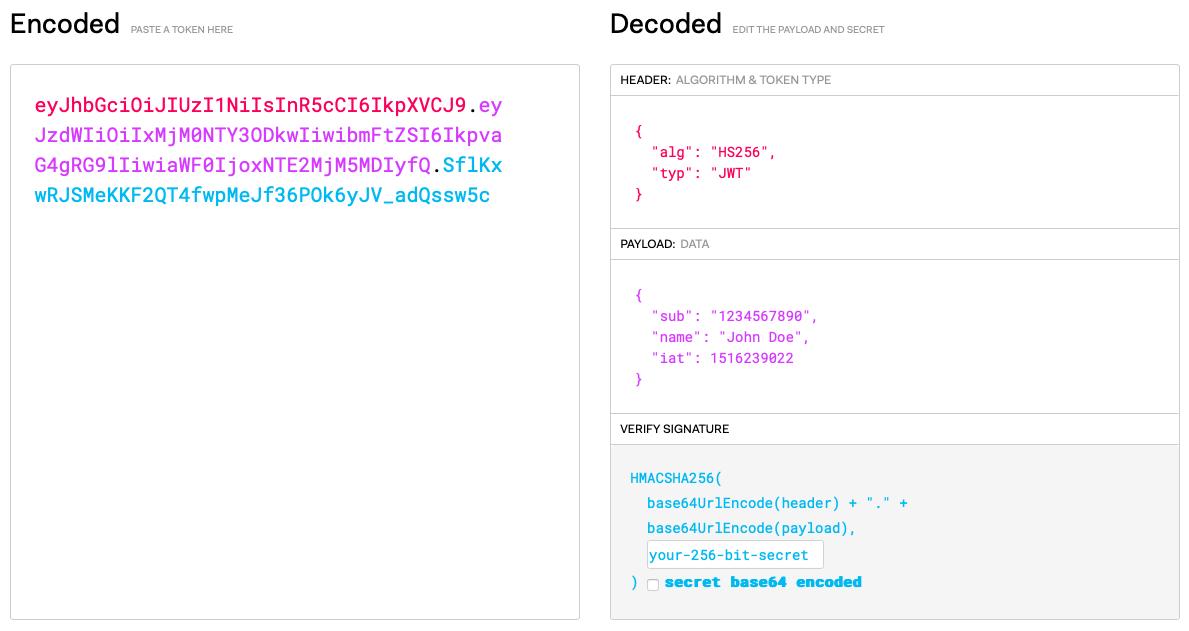
\includegraphics[width=.85\linewidth]{jwt.png}
	\caption{Vergleich von enkodiertem und dekodiertem JWT}
	\label{jwt-decoder}
\end{figure}

Dieser Standard überträgt Authentifizierungs- und Autorisierungsinformationen zwischen zwei Teilnehmern eines Netzwerks in Form einer Zeichenkette, dem Token. Diese Methode soll einen einfachen Informationsaustausch für Anmeldungen ermöglichen, ohne das eine aktive Verbindung aufrechterhalten werden muss.

Diese Eigenschaften machen JWT portabel und skalierbar. Die Übertragung ist Plattformübergreifend möglich und das Format ist kompakt. Der Server muss hier keine Sitzungsinformationen speichern, da JWT alle Informationen über die Berechtigungen enthält. Eine Manipulation ist nicht möglich, da es sonst zu Fehlern bei einer Validierung der Signatur kommt.\cite{ionos-jwt}

JWTs wirken bei Single-Sign-On (SSO) unterstützend, da der Benutzer nach einer Authentifizierung einen JWT erhält, welchen er für die Anmeldung bei Anfragen an einen Server verwenden kann.